\documentclass[bibliography=totoc,12pt,a4paper]{scrartcl}
\usepackage{amsmath, amssymb, amsthm}
\usepackage{enumerate}% schicke Nummerierung
\usepackage{graphicx}
\usepackage[english, ngerman]{babel}
\usepackage[T1]{fontenc}
\usepackage{lmodern}
\usepackage[utf8]{inputenc}
\usepackage{bigdelim}
\usepackage{multirow}
\usepackage{dsfont}
\usepackage[colorlinks=true,linkcolor=black, citecolor=black]{hyperref}
\usepackage{cite}
\usepackage[nottoc]{tocbibind}
\usepackage{empheq}
\usepackage{fancyhdr}
\usepackage{geometry}
\usepackage{lipsum}
\usepackage{tikz,pgfplots}
\usepackage{nicefrac}
\usetikzlibrary{shapes.misc}
\usetikzlibrary{matrix}
\geometry{a4paper,left=40mm,right=30mm, top=5cm, bottom=5cm} 

\def\@biblabel#1{\textcolor{red}{[#1]}}

\newtheoremstyle{linebreak}   % name
{3pt}                         % Space above
{3pt}                         % Space below
{}                            % Body font
{}                            % Indent amount 1
{\bfseries}                   % Theorem head font
{\newline}                    % Punctuation after theorem head
{.5em}                        % Space after theorem head 2
{}                            % Theorem head spec (can be left empty, meaning ‘normal’)
%\theoremstyle{linebreak}
\newtheoremstyle{exampstyle}
  {\topsep} % Space above
  {\topsep} % Space below
  {} % Body font
  {} % Indent amount
  {\bfseries} % Theorem head font
  {.} % Punctuation after theorem head
  {.5em} % Space after theorem head
  {} % Theorem head spec (can be left empty, meaning `normal')
\theoremstyle{exampstyle}
\newtheorem{defi}{Definition}%[chapter]
\newtheorem{satz}[defi]{Satz}
\newtheorem{theorem}[defi]{Theorem}
\newtheorem{propo}[defi]{Proposition}
\newtheorem{lemma}[defi]{Lemma}
\newtheorem{cor}[defi]{Korollar}
\newtheorem{bem}[defi]{Bemerkung}
\newtheorem{bsp}[defi]{Beispiel}
\newtheorem{folg}[defi]{Folgerung}
%bemerkungen oder Fließtext???
\numberwithin{equation}{section} 
 \newcommand{\newln}{\\&\quad\quad{}}
 \setlength\parindent{0pt}

\renewenvironment{abstract}
 {\small
  \begin{center}
  \bfseries \abstractname\vspace{-.5em}\vspace{0pt}
  \end{center}
  \list{}{%
    \setlength{\leftmargin}{12mm}% <---------- CHANGE HERE
    \setlength{\rightmargin}{\leftmargin}%
  }%
  \item\relax}
 {\endlist}




\begin{document}

\title{Seminar über Numerische Methoden im Machine Learning \\ Bayesianische Inferenz}

\author{Daniel Luft & Fabian Gernandt \\ Prof. Dr. V. Schulz}

  \pagestyle{empty}

  % Titelblatt der Arbeit
  \begin{titlepage}

%    \includegraphics[scale=0.45]{kit-logo.jpg}
    \vspace*{2cm} 

 \begin{center} \large 
    
    Seminarausarbeitung
    \vspace*{2cm}

    {\huge Bayesian Inference}
    \vspace*{2.5cm}

    Daniel Luft \& Fabian Gernandt
    \vspace*{6cm}


	Universität Trier
  \end{center}
\end{titlepage}
%\maketitle

  % Inhaltsverzeichnis
  \tableofcontents

\newpage

  % Ab sofort Seitenzahlen in der Kopfzeile anzeigen
  \pagestyle{headings}
  
\selectlanguage{ngerman}
\begin{abstract}
In diesem Paper möchten wir eine kurze Einführung in die Bayes Theorie im Rahmen des Machine Learnings geben, welche den Anspruch hat für Leser mit nur geringen Kenntnissen der Statistik und Wahrscheinlichkeitstheorie lesbar zu sein. Wir nutzen die Bayes Theorie um alternative numerische Problemstellungen zu klassischen Verfahren des Machine Learning zu erzeugen. Exemplarisch führen wir aufbauend auf der linearen Regression in die Bayesianische Regression ein, und erhalten die regularisierten Verfahren Ridge Regression und LASSO. Weiterhin greifen wir die Klassifizierungstechnik der Support Vector Machine (SVM) auf und geben eine Herleitung der sogenannten Least-Squares-SVM (LS-SVM) an. Weiterführend werden Möglichkeiten zur Hyperparameterschätzung, sowie der Selektion von Kernen in diesem Modell erarbeitet. Diese Techniken münden abschließend gemeinsam in einen Algorithmus zur Lösung der LS-SVM bei mehreren konkurrierenden Kernen.
\end{abstract}
\vspace{1cm}

\thispagestyle{plain}
\section{Einführung in die Bayes Theorie}

Das Maschinelle Lernen nimmt in dem Zeitalter der Digitalen Revolution eine zunehmend zentrale Rolle ein. Schon jetzt basieren zahlreiche Produkte von global Playern wie Google, Facebook, aber auch Kalashnikov und Co. auf Techniken des Maschinellen Lernens. Zu diesen Techniken zählen Klassifizierungsmethoden wie die Support Vector Machine (SVM) und sogenannte Neural Networks. Eines ihrer charakteristischen Merkmale ist die Verwendung großer Datensätze (Big Data), was zu interessanten Fragestellungen im Bereich der Mathematik und Statistik, aber auch der Informatik führt. Wir möchten in diesem Paper eine mathematisch-statistische Perspektive auf gewisse Problemklassen einnehmen, um hieraus einen erweiterten Zugang zu klassischen numerischen Problemstellungen des Machine Learning zu erhalten.

%hier vielleicht etwas mehr zur Bayes Theorie?
%Notation D= ((x,y),...)? Einheitlich? Modelltraining erwähnen oder Verweis?
%Verweise zur Relevanz/ Quellen?

Ziel ist es, bestimmte Sachverhalte mit Hilfe von Modellgleichungen abzubilden. Diese Modelle bestehen in der Regel aus Inputdaten $x \in \mathbb{R}^m$, einem Output $y \in \mathbb{R}^p$, sowie von Modellparametern, welche wir mit $\theta \in \mathbb{R}^k$ bezeichnen werden. Weiterhin werden wir Datensätze $D = (d_1, \cdots, d_n), d_i \in \mathbb{R}^l$ verwenden, um unsere Modelle zu trainieren. 

%Diagramm? Lineare Regression Vorwegnehmen, um exemplarisch zu zeigen was gemeint ist?

Hierzu wählen wir den statistischen Ansatz der sogenannten Bayes Theorie. Diese Theorie verwendet Verteilungsannahmen an Parameter $\theta$ des Modells. Solche Annahmen ermöglichen eine umfangreiche wahrscheinlichkeitstheoretische Behandlung des Modells.

Zunächst einigen wir uns auf folgende Notation von Verteilungen und Wahrscheinlichkeiten: \\
Sei $(\Omega, \mathcal{A}, \mathbb{P})$ ein hinreichend großer Wahrscheinlichkeitsraum, denn wir im Folgenden immer im Hintergrund voraussetzen werden. Weiterhin sei $\theta: \Omega \rightarrow \mathbb{R}^k$ eine Zufallsvariable. Dann bezeichnen wir mit
$\mathbb{P}(\theta) := \mathbb{P}^\theta = \mathbb{P}(\{ \theta \in \cdot \})$
das Bildmaß der Zufallsvariable $\theta$, also Ihre Verteilung.
Wir möchten hier bemerken, dass es keinen Sinn macht nach der Wahrscheinlichkeit von $\theta$ zu fragen, sondern lediglich von der Wahrscheinlichkeit dass $\theta$ bestimmte Werte annimmt. Dies ist wichtig, um Missverständnisse zu vermeiden.

Wir möchten nun in die Grundbegriffe der Bayes Theorie einführen. 
%Zitat woher die Definitionen kommen.
Die zentralen Objekte der Bayes Theorie sind die A Priori Verteilung (Prior) und die A Posteriori Verteilung (Posterior), welche durch den Satz von Bayes in Verbindung stehen. 

\begin{defi}[A Priori Verteilung]
	Sei der Modellparameter $\theta$ mit Werten im $\mathbb{R}^k$ eine Zufallsvariable. 		\\
	Dann heißt seine Verteilung $\mathbb{P}(\theta)$ \textit{A Priori Verteilung}, kurz 		\textit{Prior}. 
\end{defi}
%Quelle zur Bayes Theorie

Der Prior als Wahrscheinlichkeitsverteilung muss vor dem weiteren Arbeiten mit einem Bayesianischen Modell durch eine Annahme festgelegt werden. Es ist für sich nicht klar welcher Prior für ein gegebenes Modell sinnvoll ist, was zur Gefahr widersprüchlicher oder hinderlicher Annahmen führt. Deshalb ist vor dem Platzieren eines Priors eine gründliche Überlegung über Eigenschaften der Parameter wichtig. Verschiedene Priors führen zu verschiedenen Modellen und somit zu verschiedenen Problemklassen, weshalb auch eine entgegengesetzte Betrachtung möglich ist, bei der bei gegebener Problemklasse der zugrunde liegende Prior gesucht ist. Wir wählen den anderen Ansatz, und konstruieren Probleme bei gegebenem Prior.

Bevor wir die A Posteriori Verteilung einführen, erinnern wir an den Satz von Bayes.

\begin{theorem}[Satz von Bayes (Bayes 1763, Laplace 1812)]
	Sei $(\Omega, \mathcal{A}, \mathbb{P})$ ein Wahrscheinlichkeitsraum, seien 
	$A,B \in \mathcal{A}$ Ereignisse. Dann gilt für die bedingten Wahrscheinlichkeiten
	\begin{center}
		$\mathbb{P}(A\vert B) = \frac{\mathbb{P}(B \vert A) \mathbb{P}(A)}{\mathbb{P}				(B)}$.
	\end{center}
	Falls $\mathbb{P}(B) = 0$, so definieren wir den rechten Ausdruck als $0$.
\end{theorem}

\begin{proof}
	Mit Definition einer bedingten Wahrscheinlichkeit erhält man
	\begin{center}
		$\frac{\mathbb{P}(B \vert A) \mathbb{P}(A)}{\mathbb{P}(B)}
		= \frac{\frac{\mathbb{P}(B \cap A)}{\mathbb{P}(A)} \mathbb{P}(A)}{\mathbb{P}(B)}
		= \frac{\mathbb{P}(B \cap A)}{\mathbb{P}(B)}
		= \mathbb{P}(A\vert B)$.
	\end{center}
\end{proof}

Gegeben eines Priors möchte man nun die statistischen Daten eines Modells in die Information über die Parameter miteinfliessen lassen. Die hierzu folgende Definition ist in Anlehnung an den Satz von Bayes motiviert.

\begin{defi}[A Posteriori Verteilung]
	Sei $\theta$ ein Modellparameter mit A Priori Verteilung $\mathbb{P}(\theta)$, $D = 		(d_1, \cdots, d_n)$ ein Datenvektor. Dann definieren wir die \textit{A Posteriori 			Verteilung}, kurz \textit{Posterior}, durch
	\begin{center}
		$\mathbb{P}(\theta \vert D) := \frac{\mathbb{P}(D \vert \theta) 
		\mathbb{P}(\theta)}{\mathbb{P}(D)}$,
	\end{center}
	wobei $\mathbb{P}(D) = \int \mathbb{P}(D \vert \theta) d\mathbb{P}(\theta)$.
\end{defi}

In dem Posterior sind die kombinierte statistische Information der Annahmen, sowie der beobachteten Daten, über $\theta$ enthalten. Der Posterior besteht aus der Likelihood $\mathbb{P}(D\vert \theta)$, dem Prior $\mathbb{P}(\theta)$, sowie einem Normalisierungsfaktor $\mathbb{P}(D)$. 

Der Prozess der Berechnung des Posteriors wird oft auch \textit{Training} genannt, in diesem Kontext nennt man $D$ oft auch \textit{Trainingsdaten}. Die exakte Berechnung des Posteriors gestaltet sich bei großen Datenmengen $D$ als schwierig, besonders wenn sogenannte latente Variablen im Modell auftreten. Latente Variablen $Z$ sind Variablen, die nicht beobachtet werden können, und bei denen somit keine Daten zur Verfügung stehen. Diese treten häufig im Kontext von Bayesianischen Netzwerken, Modellen zur Textkategorisierung, rekurrenten Neuronalen Netzwerken und Sprach- sowie Texterkennung auf. Für einführende Beispiele von Modellen mit latenten Variablen im Machine Learning verweisen wir beispielhaft auf den Vortrag \cite{Latent_Variables}. 

Es bestehen Möglichkeiten zur approximativen Bestimmung des Posteriors. Als Beispiel einer statistischen Methode zur approximativen Berechnung seien hier die \textit{Markov-Chain-Monte-Carlo-Verfahren} genannt. Weiterhin gibt es analytische Approximationen, welche auf große Klassen von Verteilungen angewandt werden können. Beispielhafte Techniken sind die \textit{Expectation-Maximization-Algorithmen} und \textit{Variational-Bayes-Methoden}. Für eine Einführung in erstere, siehe \cite{Exp_Max}, für eine ausführliche Behandlung des letzteren im Rahmen des Machine Learning siehe \cite{Var_Bayes}. 


%Bsp Münzwurf??? eher nicht oder 


Wir nutzen den nun eingeführten Posterior um eine Bayesianische Art von Parameterschätzer zu definieren, den sogenannten Maximum-A-Posteriori-Schätzer. Zuvor wiederholen wir Begriff des Maximum-Likelihood-Schätzers.

\begin{defi}{Maximum-Likelihood-Schätzer}
	Sei $D = (d_1, \cdots, d_n)$ ein Datensatz, $\theta$ ein $\mathbb{R}^k$-wertiger 
	Parameter. Dann heißt der Schätzer
	\begin{center}
		$\hat{\theta}_{MLE} := \underset{\theta}{\arg \max} \mathbb{P}(D \vert \theta)$
	\end{center}
	\textit{Maximum-Likelihood-Schätzer}, kurz \textit{MLE-Schätzer}.
\end{defi}

Es sei hier erwähnt, dass ein tiefer Zusammenhang der Parameterschätzung und Optimierungsmethoden auf Mannigfaligketien besteht. Betrachtet man den Raum aller Parameter $\theta \in \Theta$ und versieht diesen mit der Fisher-Informations-Metrik, so erhält man eine riemannsche Mannigfaltigkeit, dessen Punkte als die zu den Parametern gehörigen Verteilungen interpretiert werden können. Y. Ollivier et. al. (2017) führen auf diese Weise ein Schema mit Black-Box-Ansatz zur Konstruktion von Optimierungsmethoden mit Hilfe des zur Fisher-Informations-Metrik gehörenden natürlichen Gradienten ein. Leser mit Interesse an Differentialgeometrie und numerischer Optimierung verweisen wir auf \cite{Info_Geom}. Für eine kurze Einführung in das Gebiet der Informationsgeometrie verweisen wir auf \cite{Info_Geom_intro}.

Nun führen wir in Analogie zu dem MLE-Schätzer den Bayesianischen Maximum-A-Posteriori-Schätzer ein.

\begin{defi}[Maximum-A-Posteriori-Schätzer]
	Sei $D = (d_1, \cdots, d_n)$ ein Datenvektor, $\theta$ ein $\mathbb{R}^k$-wertiger
	Parameter mit A Priori Verteilung $\mathbb{P}(\theta)$. Dann heißt der Schätzer
	\begin{center}
		$\hat{\theta}_{MAP} := \underset{\theta}{\arg \max} \mathbb{P}(\theta \vert 					D)$
	\end{center}
	\textit{Maximum-A-Posteriori-Schätzer}, kurz \textit{MAP-Schätzer}. Hierbei ist 
	$\mathbb{P}(\theta \vert D)$ der Posterior von $\theta$ gegeben $D$.
\end{defi}

Der MAP-Schätzer ist ein statistischer Schätzer, der sich von dem MLE-Schätzer dadurch unterscheidet, dass er sowohl A Priori Annahmen an die Verteilung, als auch Daten bei der Parameterschätzung berücksichtigt. Diesen Zusammenhang erkennt man an folgender Proposition:\vspace*{0,3cm}
\begin{propo}[Darstellung des MAP-Schätzers]
	Es gelten folgende Identitäten des MAP-Schätzers:
	\begin{align*}
	\hat{\theta}_{MAP}\: &\hspace{-3pt}:= \underset{\theta}{\arg \max} \mathbb{P}(\theta \vert D) \\
						&= \arg\underset{\theta \in \Theta}{\max} \frac{ \mathbb{P}(x									\vert\theta) \mathbb{P}(\theta)}{\int  \mathbb{P}(x\vert 						\theta)\text{d}\mathbb{P}(\theta)} \\
 						&= \arg\underset{\theta \in \Theta}{\max}  \mathbb{P}(x\vert 									\theta) \mathbb{P}(\theta) \\
					 	&= \arg\underset{\theta \in \Theta}{\max} \log\mathbb{P}(x\vert 								\theta) + \log \mathbb{P}(\theta)
	\end{align*}
	\label{prop:map}
\end{propo}

\begin{proof}
Definition des MAP-Schätzers und des Posteriors, sowie die Tatsache, \\ dass $\int  \mathbb{P}(x\vert \theta) \text{d}\mathbb{P}(\theta) \in \mathbb{R}$ als Skalar nicht von $\theta$ abhängt und $\log$ monoton wachsend ist.
\end{proof}

Besonders anhand der letzten Identität erkennt man, dass der MAP-Schätzer die Information der Daten $D$ im log-Likelihood-Anteil mit der A Priori-Information des log-transformierten Priors kombiniert. Diese Darstellungen werden wir im weiteren verwenden um Optimierungsprobleme. Im Wesentlichen wird es bei allen Herleitungen in den folgenden Kapiteln darum gehen, durch das Aufstellen des MAP-Schätzers in verschiedenen Situationen regularisierte oder gänzlich neue Problemstellungen und Verfahren im Machine Learning herzuleiten. Da wir nun die Grundlagen eingeführt haben, fahren wir fort mit unserem ersten nichttrivialen Anwendungsbeispiel, der Bayesianischen Regression.
%Darstellung MAP-Schätzer


%verweis zu informationsgeometrie, Herr Schulz findet das bestimmt super

%bibtex kommas hinkriegen
\newpage
\thispagestyle{plain}
\section{Bayesian Regression}

\subsection{Multiple lineare Regression}

Als erstes nicht-triviales Anwendungsbeispiel soll die Bayes Regression dienen. Dieses Gebiet ist eine Abwandlung der multiplen linearen Regression und des kleinste-Quadrate-Schätzers. Deshalb wird die klassische Problemstellung der Regression kurz wiederholt. Das grundlegende Modell der multiplen linearen Regression lautet in Matrixschreibweise
\begin{align*}
	y\;=\;X\beta+\varepsilon.
\end{align*}
Dabei ist \(y\in\mathbb{R}^n\) die abhängige Variable bzw. der Modell-Output, \(X\in\mathbb{R}^{n\times (K+1)}\) die Matrix der unabhängigen Variablen bzw. des Input-Datensatzes mit \(K\) Variablen, \(\beta\in\mathbb{R}^{K+1}\) der Modell-Koeffizientenvektor und \(\varepsilon\in\mathbb{R}^{n}\) der Fehlerterm. Für \(\varepsilon\) wird generell eine Normalverteilungsannahme gemacht. Die Fehlerterme sind demnach multivariat normalverteilt mit Mittelwert 0 und Varianz \(\sigma^2I_n\). Da die Störgrößen \(\varepsilon\) sowie die wahren \(\beta\)-Koeffizienten generell unbekannt sind, muss das Modell geschätzt werden. Der Output-Vektor mit geschätztem \(\hat{\beta}\) lautet
\begin{align*}
	\hat{y}\;=\;X\hat{\beta}.
\end{align*}
Hierbei stellt sich nun die Frage nach einem geeigneten Schätzer, der das wahre \(\beta\) möglichst genau trifft. Der bei weitem bekannteste Schätzer für \(\beta\) ist der kleinste-Quadrate-Schätzer (kQ-Schätzer oder OLS-Schätzer). Bei diesem Ansatz sollen die \(\beta\)-Koeffizienten des linearen Modells so bestimmt werden, dass die Summe der quadrierten Residuen minimal wird. Der Vektor der Residuen \(e\) ist dabei gegeben durch
\begin{align*}
	e\;=\;y-\hat{y}\;=\;y-X\hat{\beta},
\end{align*}
also die Abweichung vom gemessenen \(y\) zum geschätzten \(\hat{y}\). Die Summe der quadrierten Residuen ist dann \(e^Te\), welche als quadratische Funktion der Koeffizienten betrachtet werden kann. Es existiert somit immer ein Minimum. Dieses wird durch ableiten von \(e^Te=\left(y-X\hat{\beta}\right)^T\left(y-X\hat{\beta}\right)\) nach \(\hat{\beta}\) und anschließendes Nullsetzen bestimmt. Man erhält den (analytischen) kQ-Schätzer
\begin{align*}
	\hat{\beta}\;=\;\left(X^TX\right)^{-1}X^Ty.
\end{align*}
Dieser besitzt besondere Eigenschaften. Nach dem Gauss-Markov Theorem (vgl. \cite{Eco}, S.46-47) ist der kQ-Schätzer nun derjenige Schätzer für \(\beta\) mit der geringsten Varianz unter allen linearen und unverzerrten Schätzern (\textbf{B}est \textbf{L}inear \textbf{U}nbiased \textbf{E}stimator, \textbf{BLUE}).\\
Allerdings ist der kQ-Schätzer nicht perfekt. Die Invertierung der Matrix \(\left(X^TX\right)\) kann problematisch werden, da diese zwar mindestens positiv semidefinit ist, aber ein Eigenwert nahe 0 die Inverse schlecht konditioniert. Er trifft das wahre \(\beta\) zwar im Erwartungswert, jedoch kann dessen Varianz wegen der Invertierung unter Umständen beliebig groß und der Schätzer damit beliebig ungenau werden. Dies tritt zum Beispiel bei Multikollinearität in den Input-Daten auf, also wenn Abhängigkeiten zwischen zwei oder mehr Variablen vorliegen. Als Alternative zum kQ-Schätzer wird nun der Ridge-Schätzer betrachtet.

\subsection{Ridge-Regression}

Der \textit{Ridge-Regression-Schätzer} (auch \textit{Ridge-Schätzer}), bekannt durch \textit{Hoerl} und \textit{Kennard} (vgl. \cite{Ridge}, 1970), ursprünglich von \textit{Tikhonov} (1943), ist die wohl meist verwendete Abwandlung des kQ-Schätzers zur Regularisierung von schlecht konditionierten Problemen. Der Schätzer folgt in seiner allgemeinen Form aus der Idee, dass die Matrix \(X^TX\) durch Addition einer positiv definiten Matrix sicher positiv definit wird. Konkret lautet der Ridge-Schätzer für \(\beta\)
\begin{align*}
	\hat{\beta}_{Ridge}\;=\;\left(X^TX+\lambda I_k\right)^{-1}X^Ty.
\end{align*}
Genauer löst der Schätzer das Minimierungsproblem
\begin{align*}
	\hat{\beta}_{Ridge}\;=\; \underset{\beta}{\arg\min}\left[\left(y-X\beta\right)^T\left(y-X\beta\right)+\lambda\beta^T\beta\right],
\end{align*}
wobei der erste Summand analog zum kQ-Minimierungsproblem ist und der zweite Summand eine Nebenbedingung an die \(\beta\)-Koeffizienten darstellt. Diese werden durch die Nebenbedingung gegen 0 geschoben und somit betraglich kleiner gehalten, als beim kQ-Schätzer.\\
Obiges Zielfunktional soll nun mittels Bayes Ansatz hergeleitet werden. Die  Annahmen der multiplen linearen Regression können zunächst wie folgt interpretiert werden:
\begin{align*}
	\mathbb{P}(y_i\vert \beta)\;=\;\mathcal{N}(X_i\beta,\sigma^2),
\end{align*}
was bedeutet, dass der Output-Vektor \(y\) i.i.d. ist und als multivariat normalverteilte Zufallsvariable mit Mittelwert \(X\beta\) und Kovarianzmatrix \(\sigma^2I_n\) angesehen werden kann, was direkt aus dem Grundmodell der multiplen linearen Regression folgt.\\
Des weiteren wird nun eine a priori Annahme an die Regressionsgewichte \(\beta\) gemacht. Diese sollen nun ebenfalls normalverteilt sein. Die a priori Annahmen sind insgesamt:
\begin{enumerate}[(i)]
	\item \(\mathbb{P}(y_i\vert \beta)\;=\;\mathcal{N}(X_i\beta,\sigma^2)\)
	\item \(\beta\sim \mathcal{N}(0, \tau^2 I_k)\)
	\item \(y_i\) und \(\beta_i\) i.i.d.
\end{enumerate}
\hfill\\Mit den Annahmen folgt zum einen
\begin{align*}
	\mathbb{P}(y|\beta)&\;\overset{(\text{iii})}{=}\;\prod_{i=1}^{n}\mathbb{P}(y_i|\beta)\\
	&\;\:\overset{(\text{i})}{=}\:\:\prod_{i=1}^{n}\frac{1}{\sigma\sqrt{2\pi}}\exp\left(-\frac{\left(y_i-X_i\beta\right)^2}{2\sigma^2}\right),
\end{align*}
zum anderen
\begin{align*}
	\mathbb{P}(\beta)&\;\overset{(\text{iii})}{=}\;\prod_{i=1}^{k}\mathbb{P}(\beta_i)\\
	&\,\,\:\!\overset{(\text{ii})}{=}\:\,\prod_{i=1}^{k}\frac{1}{\tau\sqrt{2\pi}}\exp\left(-\frac{\beta_i^2}{2\tau^2}\right).\qquad\;\;\:
\end{align*}
Nun ergibt sich mit Proposition \autoref{prop:map} für den MAP-Schätzer
\begin{alignat*}{2}
	\hat{\beta}_{\text{MAP}}&\;=\;\underset{\beta}{\arg\max}&& \log\mathbb{P}(y\vert \beta) + \log \mathbb{P}(\beta) \\
	&\;=\;\underset{\beta}{\arg\max}&&\left[\log\left(\prod_{i=1}^{n}\frac{1}{\sigma\sqrt{2\pi}}\exp\left(-\frac{\left(y_i-X_i\beta\right)^2}{2\sigma^2}\right)\right)\right.\\	&\hspace{1,7cm}+&&\:\:\left.\log\left(\prod_{i=1}^{k}\frac{1}{\tau\sqrt{2\pi}}\exp\left(-\frac{\beta_i^2}{2\tau^2}\right)\right)\right]\\
	&\;=\;\underset{\beta}{\arg\max} && \left[-\sum_{i=1}^{n}\frac{\left(y_i-X_i\beta\right)^2}{2\sigma^2}-\sum_{i=1}^{k}\frac{\beta_i^2}{2\tau^2}\right]\\
	&\;=\;\underset{\beta}{\arg\max} && \left[\frac{1}{2\sigma^2}\left(-\sum_{i=1}^{n}\left(y_i-X_i\beta\right)^2-\frac{\sigma^2}{\tau^2}\sum_{i=1}^{k}\beta_i^2\right)\right]\\
	&\;=\;\underset{\beta}{\arg\min} && \left[\sum_{i=1}^{n}\left(y_i-X_i\beta\right)^2+\lambda\sum_{i=1}^{k}\beta_i^2\right]\\
\end{alignat*}
Damit erhält man das Ridge-Optimierungsproblem
\begin{align*}
	\hat{\beta}_{Ridge}\;=\;\underset{\beta}{\arg\min}\left[\left(y-X\beta\right)^T\left(y-X\beta\right)+\lambda \beta^T\beta\right].
\end{align*}
\hfill\\ Der Ridge-Schätzer besitzt die gewünschte Eigenschaft, schon bei kleinem \(\lambda\) die Varianz der Modellkoeffizienten zu reduzieren, ist aber verzerrt und besitzt als Erwartungswert nicht das wahre \(\beta\). \\
Analog dazu lassen sich weitere Schätzer herleiten. Hier soll kurz noch der LASSO-Schätzer (least absolute shrinkage and selection operator) hergeleitet werden.

\subsection{Der LASSO-Schätzer}

Analog zum Ridge-Schätzer lässt sich der LASSO-Schätzer über eine Verteilungsannahme an die \(\beta\)-Koeffizienten herleiten. Grundlage des LASSO-Schätzers ist die Überlegung, anstelle einer \(L^2\)-Regularisierung einen \(L^1\)-Term in der Nebenbedingung als Regularisierer zu verwenden. Dazu wird als Prior eine Laplace-Verteilung angesetzt. Die Dichte der Laplace-Verteilung lautet
\begin{align*}
	f_{Laplace}(x|\mu,\tau)\;=\;\frac{1}{2\tau}\exp\left(-\frac{\left|x-\mu\right|}{\tau}\right)
\end{align*}
und man wählt \(\beta\sim Laplace(0, \tau)\) als Verteilungsannahme. Nun folgt analog zum Ridge-Schätzer mittels Proposition \autoref{prop:map} für den MAP-Schätzer
\begin{alignat*}{2}
	\hat{\beta}_{\text{MAP}}&\;=\;\underset{\beta}{\arg\max}&& \log\mathbb{P}(y\vert \beta) + \log \mathbb{P}(\beta) \\
	&\;=\;\underset{\beta}{\arg\max}&&\left[\log\left(\prod_{i=1}^{n}\frac{1}{\sigma\sqrt{2\pi}}\exp\left(-\frac{\left(y_i-X_i\beta\right)^2}{2\sigma^2}\right)\right)\right.\\	&\hspace{1,7cm}+&&\:\:\left.\log\left(\prod_{i=1}^{k}\frac{1}{2\tau}\exp\left(-\frac{\left|\beta_i\right|}{\tau}\right)\right)\right]\\
	&\;=\;\underset{\beta}{\arg\max} && \left[-\sum_{i=1}^{n}\frac{\left(y_i-X_i\beta\right)^2}{2\sigma^2}-\sum_{i=1}^{k}\frac{\left|\beta_i\right|}{\tau}\right]\\
	&\;=\;\underset{\beta}{\arg\max} && \left[\frac{1}{2\sigma^2}\left(-\sum_{i=1}^{n}\left(y_i-X_i\beta\right)^2-\frac{\sigma^2}{2\tau}\sum_{i=1}^{k}\left|\beta_i\right|\right)\right]\\
	&\;=\;\underset{\beta}{\arg\min} && \left[\sum_{i=1}^{n}\left(y_i-X_i\beta\right)^2+\lambda\sum_{i=1}^{k}\left|\beta_i\right|\right]
\end{alignat*}
und man erhält das LASSO-Optimierungsproblem
\begin{align*}
	\hat{\beta}_{LASSO}\;=\;\underset{\beta}{\arg\min}\left[\left(y-X\beta\right)^T\left(y-X\beta\right)+\lambda\sum_{i=1}^{k}\left|\beta_i\right|\right].
\end{align*}
Dieser Schätzer besitzt wieder andere Eigenschaften, als der Ridge-Schätzer. Die beiden größten Unterschiede zum Ridge-Schätzer liegen darin, dass der LASSO-Schätzer zwar nur algorithmisch, z.B. mit Semismooth-Newton-Methoden, bestimmt werden kann, dafür aber die Koeffizienten genau auf 0 setzen kann, was bei der Ridge-Regression nur im Grenzfall \(\lambda\rightarrow\infty\) möglich ist.\\[0,3cm]
Die beiden vorgestellten Schätzer sollen als Einführung in die Anwendung der Bayes Theorie genügen. Als nächstes wird ein weiterführendes Beispiel betrachtet, die Least-Squares-Support Vector Machine als Alternative zur herkömmlichen Support Vector Machine.
\newpage
\thispagestyle{plain}
\section{Least-Squares-Support Vector Machine}

In diesem Abschnitt soll das Bayesian Framework auf ein bekanntes Problem angewendet werden, genauer die Klassifizierung von Daten. Es wird dabei im folgenden die Binärklassifizierung betrachtet.\\
Generell ist bei solchen Problemen immer ein Datensatz \((x_i,y_i)_{i=1,\dots,n}\) von Features \(x_i\in\mathbb{R}^{n_f}\) und Klassenzugehörigkeiten \(y_i=\pm1\) gegeben. Diese Daten werden auch Trainingsobjekte genannt. Jedes Objekt wird durch einen Vektor \(x_i\) in einem Vektorraum repräsentiert. Aufgabe der Support Vector Machine ist es nun, in diesen Raum eine Hyperebene zu finden, die als Trennfläche dient und die Trainingsobjekte in zwei Klassen teilt. Der Abstand der Vektoren, die der Hyperebene am nächsten liegen, wird dabei maximiert. Dieser breite, leere Rand soll später dafür sorgen, dass auch Objekte, die nicht genau den Trainingsobjekten entsprechen, möglichst zuverlässig klassifiziert werden.\\[0,5cm]
Beim Einsetzen der Hyperebene ist es nicht notwendig, alle Trainingsvektoren zu beachten. Vektoren, die weiter von der Hyperebene entfernt liegen, beeinflussen Lage und Position der Trennebene nicht. Die Hyperebene ist nur von den ihr am nächsten liegenden Vektoren abhängig, und auch nur diese werden benötigt, um die Ebene mathematisch exakt zu beschreiben. Diese nächstliegenden Vektoren werden nach ihrer Funktion Stützvektoren (engl. support vectors) wodurch sich der Name Support Vector Machines (SVM) erklärt. \\[0,5cm]
Weiterhin ist es wichtig zu beachten, dass eine Hyperebene nicht verbogen werden kann, weshalb die Daten zur Nutzung einer linearen Trennebene auch linear separierbar sein müssen. Da dies aber in der Realität nicht häufig der Fall ist, werden im Nachfolgenden die beiden Fälle der linear und nicht-linear trennbaren Trainingsdaten betrachtet.

\subsection{Klassische Support Vector Machine}

\subsubsection{Linear trennbare Daten}

\begin{defi}[Hyperebene]
	Eine Hyperebene im \(n\)-dimensionalen euklidischen Raum \(\mathbb{R}^n\) ist eine Teilmenge \(H\in\mathbb{R}\) der Form
	\begin{align*}
		H\;=\;\lbrace x\in\mathbb{R}^n\:|\:w^Tx+b\;=\;0\rbrace,
	\end{align*}
	wobei \(w\in\mathbb{R}^n\setminus\lbrace0\rbrace\) ein Normalenvektor der Hyperebene ist. Die Variable \(b\) wird hierbei \textit{Bias} genannt.
\end{defi}

Sind zwei Klassen von Beispielen durch eine Hyperebene voneinander linear trennbar, gibt es in der Regel unendlich viele Hyperebenen, welche beide Klassen voneinander trennen. Die SVM versucht nun, von allen möglichen trennenden Hyperebenen diejenige mit minimaler quadratischer Norm \(\|w\|^2_2\) auszuwählen, so dass gleichzeitig \(y_i\left(w^Tx_i+b\right)\geq 1\) für jedes Trainingsbeispiel \(x_i\) gilt. Dies ist äquivalent zur Maximierung des kleinsten Abstands zur Hyperebene, dem sogenannten Margin. Da hierbei keine Fehler in der Trennung zugelassen werden müssen, spricht man vor allem im Bezug zu nicht-linear trennbaren Daten auch von einem Hard-Margin. Insgesamt ergibt sich daraus der folgende Satz.

\begin{satz}[Primales SVM-Problem]
	Unter den obigen Vorüberlegungen definiert die Lösung des Minimierungsproblems
	\begin{align*}
		&\min_{w,b} \frac{1}{2}\|w\|^2_2\\
		&\text{unter } y_i\left(w^Tx_i+b\right)\geq 1
	\end{align*}
	diejenige Hyperebene, welche den Datensatz \((x_i,y_i)_{i=1,\dots,n}\) mit größtmöglichem Margin trennt. Für die namensgebenden Support Vektoren gilt hierbei Gleichheit in der Nebenbedingung. 
\end{satz}

\begin{proof}
	Siehe \cite{SVM}.
\end{proof}

Das oben beschriebene Optimierungsproblem wird normalerweise in seiner dualen Form gelöst. Diese Formulierung ist äquivalent zu dem primalen Problem, in dem Sinne, dass alle Lösungen des dualen auch Lösungen des primalen Problems sind. Die Umrechnung ergibt sich dadurch, dass der Normalenvektor \(w\) als Linearkombination von Trainingsdaten geschrieben werden kann:

\begin{align*}
	w\;=\;\sum_{i=1}^{n}\lambda_i y_i x_i
\end{align*}
Die duale Form wird mit Hilfe der Lagrange-Multiplikatoren und der Karush-Kuhn-Tucker-Bedingungen hergeleitet.

\begin{satz}[Duales SVM-Problem]
	Das primale SVM-Problem ist äquivalent zum dualen Minimierungsproblem
	\begin{align*}
		&\min_{\lambda} \frac{1}{2}\sum_{i=1}^{n}\sum_{j=1}^{n}\lambda_i\lambda_jy_iy_jx_i^Tx_j-\sum_{i=1}^{n}\lambda_i\\
		&\text{unter } \sum_{i=1}^{n}\lambda_iy_i\;=\;0,\\
		&\qquad\qquad\quad\:\:\: 0\leq\lambda_i.
	\end{align*}
\end{satz}

\begin{proof}
	Siehe \cite{SVM}.
\end{proof}

\begin{defi}[Entscheidungsfunktion]
	Um für konkrete Daten anhand der Lösung des vorherigen Minimierungsproblems entscheiden zu können, welcher Gruppe diese angehören, verwendet man die sogenannte \textit{Entscheidungsfunktion}
	\begin{align*}
		y\;=\;f(x)\;=\;\text{sign}\left(w^Tx+b\right).
	\end{align*}
	\label{defi:decision}
\end{defi}
Je nachdem, wo sich die Datenpunkte relativ zur Hyperebene befinden (also oberhalb oder unterhalb), ergibt die Anwendung der Hyperebenengleichung einen positiven oder negativen Wert, wobei nach Anwendung der Vorzeichenfunktion nur noch \(\pm1\) bleibt. Für Objekte, die genau auf der Trennebene liegen, wird der Wert zu \(0\).

\subsubsection{Nicht-linear trennbare Daten}

Um dem Problem der Nicht-linearen Trennbarkeit beizukommen, werden Schlupfvariablen \(e_i\) für jeden Datenpunkt \(x_i\) eingeführt. Diese sollen Fehler in der Nebenbedingung ausgleichen, wodurch Punkte im Margin selbst und sogar auf der falschen Seite der Hyperebene liegen können. Da die Verletzungen der Nebenbedingung möglichst klein gehalten werden sollen, werden die Schlupfvariablen in das Minimierungsproblem aufgenommen.

\begin{satz}[Primales SVM-Problem mit Soft-Margin]
	Unter den bei Soft Margin zulässigen Fehlern in der Trennung definiert die Lösung des Minimierungsproblems
	\begin{align*}
		 &\min_{w,b} \frac{1}{2}\|w\|^2_2 + \xi\sum_{i=1}^{n}e_i\\
		 &\text{unter } y_i\left(w^Tx_i+b\right)\geq 1-e_i,\\
		 &\qquad\qquad\qquad\quad\:\:\:\:  0\leq e_i,\\
		 &\qquad\qquad\qquad\quad\:\:\:\:  0< \xi
	\end{align*}
	diejenige Hyperebene, welche den Datensatz \((x_i,y_i)_{i=1,\dots,n}\) unter Zulässigkeit von Fehlern mit größtmöglichem Margin trennt.
\end{satz}

\begin{proof}
	Siehe \cite{SVM}.
\end{proof}

\begin{bem}
	Für die Support Vektoren gilt Gleichheit in der Nebenbedingung und \(e_i=0\). Für Datenpunkte, die innerhalb des Margin liegen, gilt \(e_i>0\) und Gleichheit in der Nebenbedingung.
\end{bem}

Wie schon beim linear-trennbaren Datensatz wird das Minimierungsproblem in seiner dualen Form gelöst.

\begin{satz}[Duales SVM-Problem mit Soft-Margin]
	Das primale SVM-Problem mit Soft Margin ist äquivalent zum dualen Minimierungsproblem
	\begin{align*}
		&\min_{\lambda} \frac{1}{2}\sum_{i=1}^{n}\sum_{j=1}^{n}\lambda_i\lambda_jy_iy_jx_i^Tx_j-\sum_{i=1}^{n}\lambda_i\\
		&\text{unter } \sum_{i=1}^{n}\lambda_iy_i\;=\;0,\\
		&\qquad\quad\:\:\: 0\leq\lambda_i\leq\xi.
	\end{align*}
\end{satz}

\begin{proof}
	Siehe \cite{SVM}.
\end{proof}

\subsubsection{Nicht-lineare Erweiterung mit Kernelfunktionen}

Die zuvor behandelten Darstellungen der SVM klassifizieren die Daten mittels einer linearen Funktion. Diese ist jedoch nur optimal, wenn auch das zu Grunde liegende Klassifikationsproblem linear ist. In vielen Anwendungen ist dies aber nicht der Fall. Ein möglicher Ausweg ist, die Daten in einen Raum höherer Dimension abzubilden. SVMs zeichnen sich dadurch aus, dass sich diese Erweiterung elegant einbauen lässt. Dazu benutzt man Transformationsfunktionen der Form
\begin{align*}
	\varphi \colon \mathbb {R} ^{d_{1}}\rightarrow \mathbb {R} ^{d_{2}},\quad x \mapsto \varphi (x).
\end{align*}
Dabei gilt \(d^1<d^2\), was die Anzahl möglicher trennender Abbildungen erhöht. Die Funktion \(\varphi\) ist allerdings aufwändig zu bestimmen, weshalb man den sogenannten \textit{Kernel-Trick} verwendet. In der dualen Formulierungen des Optimierungsproblems gehen die Datenpunkte \(x_i\) nur in Skalarprodukten ein. Um den Rechenaufwand zu reduzieren ersetzt man daher \(x_i^Tx_j\) durch \(\varphi(x_i)\varphi(x_j)\) und verwendet eine positiv definite \textit{Kernelfunktion}
\begin{align*}
	K(x_{i},x_{j})=\varphi (x_{i})^T\varphi (x_{j}).
\end{align*}
Dadurch kann eine Hyperebene in einem hochdimensionalen Raum implizit berechnet werden. Die Entscheidungsfunktion ergibt sich dabei direkt zu
\begin{align*}
	y\;=\;f(x)&\;=\;\text{sign}\left(\sum_{k=1}^{n}\lambda_ky_k\varphi(x_k)^T\varphi(x)+b\right)\\
	&\;=\;\text{sign}\left(\sum_{k=1}^{n}\lambda_ky_kK\left(x_k,x\right)+b\right),
\end{align*}
wenn man in Definition \autoref{defi:decision} mit \(w=\underset{k=1}{\overset{n}{\sum}}\lambda_ky_k\varphi(x_k)\) substituiert.\\[0,3cm]

Geeignete Kernelfunktionen sind zum Beispiel:
\begin{alignat*}{2}
	K(x,y)&\;=\;x^Ty && (\text{linear})\\
	K(x,y)&\;=\;\left(x^Ty+c\right)^d && (\text{polynomial})\\
	K(x,y)&\;=\;\exp \left(-{\tfrac {||x-y||^{{2}}}{2\sigma ^{{2}}}}\right) \qquad&& (\text{radial basis function, RBF})
\end{alignat*}

Andere Kernelfunktionen und weiterführende Untersuchungen sind zu finden in \cite{Kernel}.

\subsection{Least-Squares-SVM}

Wie zu Anfang des Kapitels erwähnt soll nun eine SVM mit Bayes-Framework hergeleitet werden. Dazu betrachtet man die Entscheidungsfunktion in allgemeiner Darstellung mit Kernelfunktion als Modellfunktion. Hierbei sind \(w\) und \(b\) Modellparameter, für welche nun a priori Verteilungsannahmen gemacht werden, um den MAP-Schätzer nach Proposition \autoref{prop:map} bestimmen zu können. Zusätzlich wird ein Parameter \(e\) eingeführt, welcher nun die Abweichung der Datenpunkte von der Hyperebene bzw. vom Rand des Margin darstellt. Die Annahmen an \(w\), \(b\) und die Abweichungen \(e_i\) lauten konkret:
\begin{enumerate}[(i)]
	\item \(w\) ist multivariat normalverteilt mit \(w\sim\mathcal{N}\left(0,\frac{1}{\mu}I_{n}\right)\).
	\item \(b\) ist normalverteilt mit \(b\sim\mathcal{N}\left(0,\sigma_b^2\right)\) und es gilt \(\sigma_b^2\rightarrow\infty\). Damit ist \(b\) im Grenzfall unbeschränkt gleichverteilt.
	\item \(w\) und \(b\) sind stochastisch unabhängig.
	\item Die Abweichungen \(e_i=1-y_i\left(w^T\varphi\left(x_i\right)+b\right)\) sind normalverteilt mit \(e_i\sim\mathcal{N}\left(0,\frac{1}{\xi}\right)\) und i.i.d.
	\item Der Datensatz \(D\) ist i.i.d.
\end{enumerate}
Die Annahme (i) erfolgt dabei aus ähnlichen Überlegungen, wie bei der Ridge Regression (Kapitel 2). Die Koeffizienten von \(w\) sollen demnach nicht zu groß werden, aber auch für den Prior ergeben sich Vereinfachungen durch die Normalverteilung.
Voraussetzung (ii) stellt dar, dass für \(b\) eine uniforme Annahme über die Verteilung gemacht wird, also keine Vorinformation in den Prior einfließen soll. Da eine herkömmliche Gleichverteilung jedoch beschränkt ist, verwendet man diesen Zugang.\\
Annahmen (iii) und (v) dienen zur Vereinfachung der a priori Verteilungen und ermöglichen erst deren Berechnung (s. u.). Die Forderung (iv) legt die Fehler \(e_i\) als Normalverteilt fest, aus ähnlichen Gründen wie bei (i). Durch die Gleichheitsbedingung wird zudem klar, dass der Fehlerterm für alle Datenobjekte, welche nicht auf dem Margin liegen, ungleich 0 ist und somit alle Datenpunkte im Minimierungsproblem betrachtet werden. Dies kann als multiple Regression in den Abweichungen \(e_i\) interpretiert werden und ist wohl der größte Unterschied zur klassischen SVM.\\
Die in den Forderungen auftretenden Variablen \(\mu\) und \(\xi\) sind sogenannte Hyperparameter, da sie hierarchisch über den Modellparametern stehen. \(\sigma_b^2\) ist ebenfalls ein Hyperparameter, fällt aber letztendlich durch den Grenzübergang weg. Mit diesen Annahmen folgt nun für den gemeinsamen Prior von \(w\) und \(b\):
\begin{align*}
	\mathbb{P}\left(w,b\:|\:\mu,\xi,K\right)&\;\overset{(\text{iii})}{=}\;\mathbb{P}\left(w\:|\:\mu,\xi,K\right)\cdot\mathbb{P}\left(b\:|\:\mu,\xi,K\right)\\
	&\!\!\:\overset{(\text{i}),(\text{ii})}{\propto}\;\exp\left(-\frac{\mu}{2}w^Tw\right)\exp\left(-\frac{b^2}{2\sigma_b^2}\right)\\
	&\!\overset{\sigma_b^2\rightarrow\infty}{\longrightarrow}\exp\left(-\frac{\mu}{2}w^Tw\right)
\end{align*}
Weiterhin gilt:
\begin{align*}
	\mathbb{P}\left(D\:|\:w,b,\mu,\xi,K\right)&\;\overset{(\text{v})}{=}\;\prod_{i=1}^{n}\mathbb{P}\left(x_i,y_i\:|\:w,b,\mu,\xi,K\right)\\
	&\,\overset{(\text{iv})}{\propto}\:\prod_{i=1}^{n}\mathbb{P}\left(e_i\:|\:w,b,\mu,\xi,K\right)\\
	&\,\overset{(\text{iv})}{\propto}\;\exp\left(-\frac{\xi}{2}\sum_{i=1}^{n}e_i^2\right)
\end{align*}
Damit ergibt sich mit Proposition \autoref{prop:map}
\begin{align*}
	\left(\hat{w}_{MAP},\hat{b}_{MAP}\right)&\;=\;\underset{w,b}{\arg\max}\:\mathbb{P}\left(w,b\:|\:D,\mu,\xi,K\right)\\
	&\;=\;\underset{w,b}{\arg\max}\:\log\mathbb{P}\left(w,b\:|\:\mu,\xi,K\right)+\log\mathbb{P}\left(D\:|\:w,b,\mu,\xi,K\right)\\
	&\;=\;\underset{w,b}{\arg\max}\:\left(-\frac{\mu}{2}w^Tw-\frac{\xi}{2}\sum_{i=1}^{n}e_i^2\right)\\
	&\;=\;\underset{w,b}{\arg\min}\:\left(\frac{\mu}{2}w^Tw+\frac{\xi}{2}\sum_{i=1}^{n}e_i^2\right)
\end{align*}
Insgesamt erhält man den folgendem Satz.
\begin{satz}[Least-Squares-SVM]
	Betrachte ein SVM Problem mit i.i.d. Daten \(D=(x_i,y_i)_{i=1,...,n}\). Weiterhin seien die Parameter \(w\in \mathbb{R}^n, b\in \mathbb{R}\) stochastisch unabhängig und es gelten die a priori Verteilungen:
	\begin{align*}
	&w \sim \mathcal{N}(0,\frac{1}{\mu}I_{n_f})\: \text{ und } \: b \sim \mathcal{N}(0, \sigma_b^2).
	\end{align*}
	Weiterhin sei der Fehler \(e_i =  1 - y_i(w^T \phi(x_i) +b)\) normalverteilt mit \(e_i \sim \mathcal{N}(0,\frac{1}{\xi})\). Dann sind die \(e_i\) i.i.d. und für \(\sigma_b^2 \rightarrow \infty\) gilt:
	\begin{align*}
	\left(\hat{w}_{MAP},\hat{b}_{MAP}\right)  \;=\; &\underset{w,b}{\arg \min}\: \frac{\mu}{2}w^Tw + \frac{\xi}{2}\underset{i=1}{\overset{n}{\sum}}e_i^2\\
	&\text{unter } e_i = 1 - y_i(w^T \phi(x_i) +b),\quad i=1,\dots,n
	\end{align*}
\end{satz}
\begin{proof}
	Der Beweis folgt aus den obigen Vorüberlegungen.
\end{proof}
Zur Lösung des Problems wird zunächst noch durch \(\mu\) geteilt und mit \(\gamma=\nicefrac{\xi}{\mu}\) substituiert. Da \(n\) Nebenbedingungen mit Gleichheit vorliegen, kann sofort die Lagrangefunktion aufgestellt werden. Diese lautet
\begin{align*}
	\mathcal{L}(w,b,e;\lambda)&\;=\;\frac{1}{2}w^Tw+\frac{\gamma}{2}\sum_{i=1}^{n}e_i^2-\sum_{i=1}^{n}\lambda_i\left(y_i\left(w^T\varphi(x_i)+b\right)-1+e_i\right).
\end{align*}
Partielles differenzieren ergibt die notwendigen  Optimalitätsbedingungen:
\begin{alignat*}{4}
	\text{(i)}&\qquad \frac{\partial \mathcal{L}}{\partial w} &&\;=\;0 && \quad\Leftrightarrow\quad w\;=\;\sum_{k=1}^{n}\lambda_ky_k\varphi(x_k) && \\[0,3cm]
	\text{(ii)}&\qquad \frac{\partial \mathcal{L}}{\partial b} &&\;=\;0 && \quad\Leftrightarrow\quad \sum_{k=1}^{n}\lambda_ky_k\;=\;0 && \\[0,3cm]
	\text{(iii)}&\qquad \frac{\partial \mathcal{L}}{\partial e_i} &&\;=\;0 && \quad\Leftrightarrow\quad \lambda_i\;=\;\gamma e_i, && i\;=\;1,\dots,n\\[0,3cm]
	\text{(iv)}&\qquad \frac{\partial \mathcal{L}}{\partial \lambda_i} &&\;=\;0 && \quad\Leftrightarrow\quad 1\;=\;y_i\left(w^T\varphi(x_i)+b\right)+e_i,\quad && i\;=\;1,\dots,n
\end{alignat*}
Nun werden \(w\) und \(e\) in (iv) eliminiert. Übrig bleibt das Gleichungssystem
\begin{align*}
	0&\;=\;\sum_{k=1}^{n}\lambda_ky_k\\
	1&\;=\;\sum_{k=1}^{n}\left[\lambda_ky_ky_i\varphi(x_k)^T\varphi(x_i)\right]+y_ib+\gamma^{-1}\lambda_i,\quad i=1,\dots,n
\end{align*}
In Matrixschreibweise lässt sich das LGS wie folgt darstellen:
\begin{align*}
	\begin{bmatrix}
		0& y^T \\[0,5cm]
		y& \Omega+\gamma^{-1}I_n
	\end{bmatrix}
	\begin{bmatrix}
		b \\[0,2cm]
		\lambda
	\end{bmatrix}\;=\;
	\begin{bmatrix}
		0 \\[0,2cm] 
		1_n
	\end{bmatrix},
\end{align*}
wobei
\begin{align*}
	y &\;=\;(y_1,\dots,y_n)^T,\\
	1_n &\;=\;(1,\dots,1)^T\in\mathbb{R}^n,\\
	\lambda &\;=\;(\lambda_1,\dots,\lambda_n)^T,\\
	\Omega_{ij} &\;=\;y_iy_j\varphi(x_i)^T\varphi(x_j)\;=\;y_iy_jK(x_i,x_j), \quad i,j=1,\dots,n.
\end{align*}
Die Einträge von \(\Omega\) sind dabei die Anwendung der Kernelfunktion \(K\) auf zwei Datenpunkte \(x_i\) und \(x_j\) multipliziert mit \(1\), wenn die Datenobjekte zur selben Klasse gehören, bzw. mit \(-1\), wenn dies nicht der Fall ist. Hierbei wird wie bei der klassischen SVM die Anwendung der schwer zu bestimmenden Transformationsfunktion \(\varphi\) durch die  Kernelfunktion \(K\) ersetzt.\\
Wie zuvor bei der SVM wird hier das duale Minimierungsproblem gelöst, im Gegensatz dazu liegt hier aber ein lineares statt eines quadratischen Programms vor, welches recht einfach gelöst werden kann. Da allerdings die Umrechnung von \(\lambda\) nach \(w\) das anwenden der Transformationsfunktion \(\varphi\) erfordert, wird darauf verzichtet und die Trennebene in ihrer dualen Form dargestellt.\vspace*{-0,3cm}
\begin{figure}[h]
	\begin{center}	
	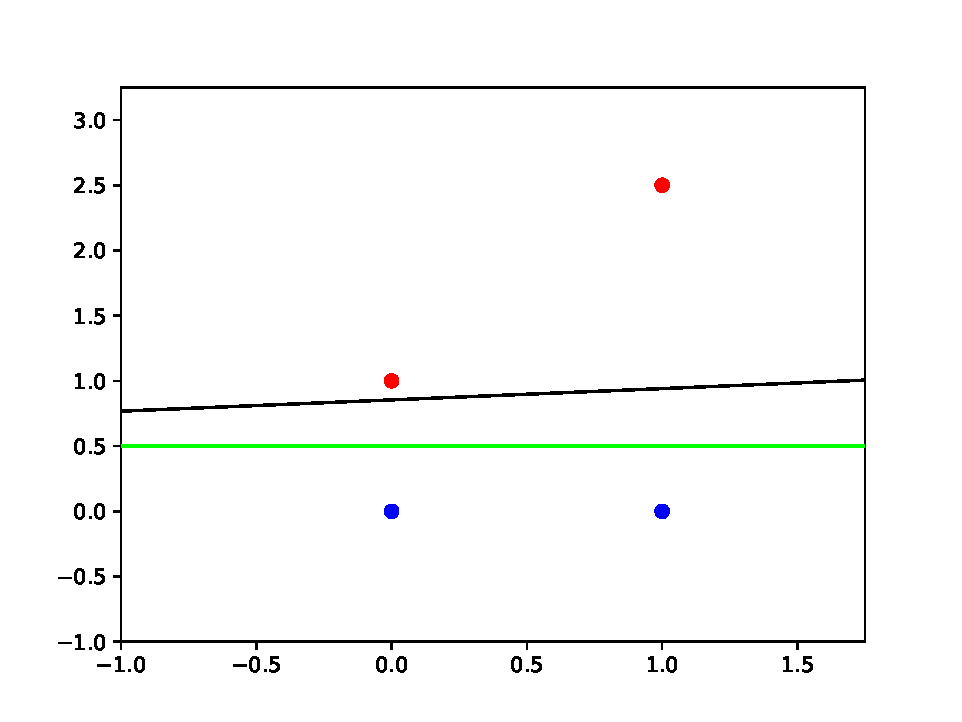
\includegraphics[scale=0.6]{SVMS.pdf}
	\end{center}
	\caption{Vergleich SVM und LS-SVM: In grün eingezeichnet ist die Trennebene der SVM, in schwarz die Trennebene der LS-SVM.}
	\label{fig:SVMS}
\end{figure}

In \autoref{fig:SVMS} wird der Unterschied zwischen den beiden Vorgehensweisen deutlich. Die grüne Linie markiert dabei die Trennebene der SVM und ist in diesem Beispiel sehr einfach nachzuvollziehen. Der Margin soll maximal werden, was bedeutet, dass die drei unten gelegenen Punkte die Support Vektoren bilden und die Ränder des Margin und dessen Breite definieren.\\
Die schwarze Linie ist die Trennebene der LS-SVM und verdeutlicht den Einfluss des oberen roten Punkts auf die Hyperebene. Würden noch weitere Punkte in die rote Klasse hinzugefügt, welche weit entfernt von der blauen Klasse liegen, so würde die Trennebene weiter nach oben und eventuell über den Punkt \(\left(0,1\right)\) hinausgeschoben, so dass dieser dann fehlerhaft klassifiziert wird.\\ 
Für weitere Theorie zur LS-SVM wird auf \cite{LS-SVM_b} verwiesen.
%%%%%%%%%%%%%%%%%%%%%%%%%%%%%
%Algorithmen zur Lösung???

%Schreibweise: Kernel oder Kerne??

%SKALARES PROBLEM?

%Verweis auf voriges Kapitel + Klärung der Begriffe n_f, N_eff nicht vergessen!

%Ausblick   + Algorithmus (evtl extra Kapitel mit sachen zur implementierung und bildern)

%diagramme nicht vergessen
%%%%%%%%%%%%%%%%%%%%%%%%%%%%%
\newpage
\thispagestyle{plain}
\section{Hyperparameterschätzung \& Kernelselektion}
\subsection{Hyperparameterschätzung}

Nachdem wir nun in dem vorangehenden Kapitel gesehen haben wie man die LS-SVM und ihr duales Problem herleitet, knüpfen wir darauf aufbauend an und leiten mögliche Arten der Hyperparameterschätzung und der Kernelselektion her. \\
Die Bayesianische Statistik ermöglicht eine rigorose Behandlung von fast beliebig komplexen statistischen Modellen durch A Priori Annahmen an Hyperparameter und deren Parameterabhängigkeit. Wir folgen weiterhin dem Ansatz aus \cite{LS-SVM} das Problem der Hyperparameterinferenz durch das Nutzen der so entstehenden MAP-Schätzer herzuleiten.

Zunächst betrachten wir erneut unsere LS-SVM Gleichung:

\begin{center}
	$(\hat{w}_{MAP},\hat{b}_{MAP})  = \underset{w,b}{\arg \min \hspace{0.1cm}} 					 \frac{\mu}{2}w^Tw + \frac{\xi}{2}\underset{i=1}{\overset{n}{\sum}}e_i^2$
	unter $e_i = 1 - y_i(w^T \phi(x_i) +b)$
\end{center}

Wir machen folgende Annahmen an die Verteilung der Hyperparemter $\mu, \xi >0$:

\begin{enumerate}[(i)]
	\item $\log(\mu) \sim \mathcal{N}(0, \sigma_\mu^2), \log(\xi) \sim \mathcal{N}(0, 				  \sigma_\xi^2)$ 
	\item $\log(\mu), \log(\xi)$ stochastisch unabhängig
	\item $\sigma_\mu^2, \sigma_\xi^2 \rightarrow \infty$.
\end{enumerate}

Die Annahmen sind dadurch zu rechtfertigen, dass als log-normalverteilte Zufallsvariablen die positiven Werte von $\mu$ und $\xi$ respektiert werden. Der Grenzwert der Varianzen $\sigma_\mu^2, \sigma_\xi^2 \rightarrow \infty$ wird dadurch gerechtfertigt, dass man eine uniforme Annahme über die Verteilung von $\mu$ und $\xi$ machen möchte, d.h. keine Vorinformation über ihre Werte verwenden will. Weiterhin wird die stochastische Unabhängigkeit die rechnerische Herleitung des Minimierungsproblems ermöglichen.

\begin{figure}
\centering
\begin{tikzpicture}
	\tikzstyle{sum} = [draw, circle, minimum size=0.8cm, node distance=1.75cm]
	\tikzstyle{block} = [draw, rectangle, minimum width = 2.75cm, minimum height = 0.5cm]
	\node [sum] (y) at (2,-3) {$y$};
	\node [sum] (eps) at (0,0) {$e$}; 
	\node [sum] (X) at (2,0) {$X$}; 
	\node [sum] (w) at (4,0) {$w,b$};
	\node [block, fill=white] (M) at (2, -1.5) {$y = \text{sign}(w^T \varphi(x) + b)$};
	\node [block, text width=3.5cm] (alpha) at (4,1.75) {$w \sim \mathcal{N}(0,\frac{1}{\mu}I_{n_f})$\\ $b \sim \mathcal{N}(0,\sigma^2_b)$};

	\draw[->,thick] (eps) -- (M);
	\draw[->,thick] (w) -- (M);
	\draw[->,thick] (X) -- (M);
	\draw[->,thick] (M) -- (y);
	%\draw[->,thick] (X) -- (y) node[block, midway, fill=white] {$y = Xw+\varepsilon$};
	\draw[->,thick] (alpha) -- (w);
	\node [block, text width=2.5cm] (lambda) at (0,2) {$e_i \sim \mathcal{N}(0,\frac{1}{\xi})$};
	\draw[->,thick] (lambda) -- (eps);
 
	\node [sum] (mu) at (4,3) {$\mu$};
	\node [sum] (xi) at (0,3) {$\xi$};
	\draw[->, thick] (xi) -- (lambda);
	\draw[->, thick] (mu) -- (alpha);		
	
	\node [block, text width=3.5cm] (vert_mu) at (4,4) {$\log(\mu) \sim \mathcal{N}(0,\sigma_\mu^2)$};		
	\node [block, text width=3.5cm] (vert_xi) at (0,4) {$\log(\xi) \sim \mathcal{N}(0,\sigma_\xi^2)$};	
	
	\draw[->, thick] (vert_mu) -- (mu);
	\draw[->, thick] (vert_xi) -- (xi);	
	
\end{tikzpicture}
\caption{Zusammenfassung der Verteilungs- und Modellannahmen}
\end{figure}
\newpage
Zunächst stellen wir über den Posterior $\mathbb{P}(\log \mu, \log \xi \vert D, K)$ mit Hilfe der Annahmen fest, dass

\begin{align*}
		& \mathbb{P}(\log(\mu), \log(\xi)\vert D, K)\\
	   &\;=\; \frac{\mathbb{P}(D\vert \log(\mu),\log(\xi),K)\mathbb{P}(\log(\mu), \log(\xi) 			  \vert K)}{\mathbb{P}(D\vert K)}  \\
\propto & \mathbb{P}(D\vert \log(\mu),\log(\xi),K)\exp(-\frac{x^2}{2\sigma_							  \mu^2})\exp(-\frac{x^2}{2\sigma_\xi^2})\\
\rightarrow & \mathbb{P}(D\vert \log(\mu),\log(\xi),K).
\end{align*}

Somit reicht es zum Aufstellen des MAP-Schätzers die Likelihood  $\mathbb{P}(D\vert \log(\mu),\log(\xi),K)$ gegeben der Hyperparameter $\mu, \xi$ zu betrachten. Diese Likelihood, und damit $\mathbb{P}(\log(\mu), \log(\xi)\vert D, K)$, lässt sich weiter mit Hilfe der MAP-Schätzer $(\hat{w}_{MAP}, \hat{b}_{MAP})$ darstellen, was wir in folgendem Lemma zusammenfassen.

\begin{lemma}[Darstellung der A Postiori Wahrscheinlichkeit]

Es gelten die zu Beginn des Kapitels getroffenen Annahmen an $\mu, \xi$. Dann folgt

\begin{align*}
	\mathbb{P}(\log(\mu), \log(\xi)\vert D, K) \propto\; & \mathbb{P}(D\vert \log(\mu),			\log(\xi),K) \\
	\propto\; & \frac{\sqrt{\mu^{n_f} \xi^n}}	{\sqrt{\det H}} \exp(- \mathcal{J}(\hat{w}			_{MAP},\hat{b}_{MAP})),
\end{align*}

wobei 
\begin{center}
	$\mathcal{J}(w,b) = \frac{\mu}{2}w^T w + \frac{\xi}{2}\overset{n}{\underset{i=1}			{\sum}} e_i ^2 \text{ und } H = \begin{pmatrix}
	\frac{\partial^2 \mathcal{J}}{\partial w^2 } & \frac{\partial^2 \mathcal{J}}				{\partial w \partial b } \\
	\frac{\partial^2 \mathcal{J}}{\partial b \partial w } & \frac{\partial^2 					\mathcal{J}}{\partial b^2 }
	\end{pmatrix}.$
\end{center}

\end{lemma}
%VERWEIS AUF VORIGES KAPITEL, GLEICHUNGEN WIE IN DEM LEVELS PAPER

\begin{proof}
Die erste Proportionalität wurde vor Beginn des Lemmas gezeigt, für die zweite siehe \cite{LS-SVM}.
\end{proof}

An dieser Stelle wäre es schon möglich das Optimierungsproblem für die Hyperparameterinferenz zu formulieren, was aufgrund der Determinante $\det H$ zu keiner befriedigenden Ausdruck führt. Dem entgegnen Gestel, Suykens et. al. durch folgende Darstellung der Determinante:

\begin{lemma}[Darstellung der Determinante der Hessematrix]
Betrache die aus dem LS-SVM Problem stammenden Ausdrücke 
\begin{center}
	$\mathcal{J}(w,b) = \frac{\mu}{2}w^T w + \frac{\xi}{2}\overset{n}{\underset{i=1}			{\sum}} e_i ^2 \text{ und } H = \begin{pmatrix}
	\frac{\partial^2 \mathcal{J}}{\partial w^2 } & \frac{\partial^2 \mathcal{J}}				{\partial w \partial b } \\
	\frac{\partial^2 \mathcal{J}}{\partial b \partial w } & \frac{\partial^2 					\mathcal{J}}{\partial b^2 }
	\end{pmatrix}.$
\end{center}

Dann gilt

\begin{center}
	$\det(H) = n \mu^{n_f - N_{eff}} \xi \underset{i=1}{\overset{N_{eff}}{\prod}}(\mu + 			\xi \lambda_i)$,
\end{center}

wobei $N_{eff}$ die Anzahl der Eigenwerte $\lambda_i$ ungleich Null der zentrierten Matrix $M \Omega M$ mit
\begin{center}
	$\Omega_{i,j} = K(x_i, x_j)$ und $M = I_n + \frac{1}{n} 1_v 1_v^T$ ist.
\end{center}
\end{lemma}

\begin{proof}
Siehe \cite{LS-SVM}, Appendix B.
\end{proof}

Beide darstellenden Lemmas lassen sich nun bei einem MAP-Schätzer Ansatz kombinieren und ergeben eines der Hauptresultate zur LS-SVM:


\begin{theorem}[Hyperparameterinferenz der LS-SVM]

Seien die Voraussetzungen an a priori Verteilungen wie zu Beginn des Kapitels.\\
(i) Dann sind die MAP-Schätzer der Hyperparameter $\mu, \xi$ gegeben durch

\begin{align*}
	(\hat{\mu}_{MAP}, \hat{\xi}_{MAP}) &\;=\; \underset{\mu, \xi}{\arg \min}  \hspace{0.2cm}		\mathcal{J}(\hat{w}_{MAP}, \hat{b}_{MAP}) + \frac{1}{2}\sum_{i=1}^{N_{eff}}\log(\mu 		+ \xi \lambda_i) \\
	 & \hspace{0.8cm}- \frac{N_{eff}}{2}\log(\mu) - \frac{n -1 }{2}\log(\xi)\\
	&\;=:\; \underset{\mu, \xi}{\arg \min} \hspace{0.2cm}	\mathcal{J}_\text{hyp}(\mu, \xi)
\end{align*}



mit dem Ausgangsfunktional der LS-SVM 
$\mathcal{J}(w,b) = \frac{\mu}{2}w^T w + \frac{\xi}{2}\overset{n}{\underset{i=1}{\sum}} e_i ^2$,
sowie den nichttrivialen Eigenwerten $\lambda_i$ der zentrierten Kernelmatrix.

(ii) Weiterhin sind die partiellen Ableitungen des Zielfunktionals gegeben durch

\begin{align*}
	\frac{\partial \mathcal{J}_\text{hyp}}{\partial \mu} &\;=\; \hat{w}_{MAP}^T \hat{w}			_{MAP} + \frac{1}{2} \overset{N_{eff}}{\underset{i=1}{\sum}} \frac{1}{\mu + \xi 			\lambda_i} - \frac{N_{eff}}{2\mu} \\
    \frac{\partial \mathcal{J}_\text{hyp}}{\partial \xi} &\;=\; \overset{n}						{\underset{i=1}{\sum}}( y_i - (\hat{w}_{MAP}^T \varphi(x_i) + \hat{b}_{MAP}))^2 + \overset{N_{eff}}{\underset{i=1}{\sum}} \frac{\lambda_i}{\mu + \xi \lambda_i} - \frac{N-1}{2\xi}.
\end{align*} 
\end{theorem}

\begin{proof}
Wir verwenden die beiden vorausgegangenen Lemmata und erhalten durch einsetzen und der Definition des MAP-Schätzers, sowie negativer log-Transformation:
\begin{align*}
	(\hat{\mu}_{MAP}, \hat{\xi}_{MAP}) 
	&\;=\; \underset{\mu, \xi}{\arg \max} \mathbb{P}(\mu, \xi \vert D, K) \\
	&\;=\; \underset{\mu, \xi}{\arg \max} \mathbb{P}(\log(\mu) \log(\xi) \vert D, K) \\
	&\;=\; \underset{\mu, \xi}{\arg \max} \mathbb{P}(D \vert \log(\mu), \log(\xi), K) \\
	&\;=\; \underset{\mu, \xi}{\arg \max} \frac{\sqrt{\mu^{n_f} \xi^n}}	{\sqrt{\det H}} 				\exp(- \mathcal{J}(\hat{w}_{MAP},\hat{b}_{MAP})) \\
	&\;=\; \underset{\mu, \xi}{\arg \max} \frac{\sqrt{\mu^{n_f} \xi^n}}	{\sqrt{n \mu^{n_f - 			N_{eff}} \xi \underset{i=1}{\overset{N_{eff}}{\prod}}(\mu + 			\xi 				\lambda_i)}} \exp(- \mathcal{J}(\hat{w}_{MAP},\hat{b}_{MAP})) \\
	&\;=\; \underset{\mu, \xi}{\arg \max} \frac{\sqrt{\mu^{N_{eff}} \xi^{n-1}}}	{\sqrt{ 				\underset{i=1}{\overset{N_{eff}}{\prod}}(\mu + 	\xi	\lambda_i)}} \exp(- 					\mathcal{J}(\hat{w}_{MAP},\hat{b}_{MAP})) \\
	&\;=\; \underset{\mu, \xi}{\arg \min}  \hspace{0.2cm} \mathcal{J}(\hat{w}_{MAP}, 			   	 	\hat{b}_{MAP}) + \frac{1}{2}\sum_{i=1}^{N_{eff}}\log(\mu + \xi \lambda_i)\\
	 & \hspace{0.8cm}- \frac{N_{eff}}{2}\log(\mu) - \frac{n -1 }{2}\log(\xi),
\end{align*}

was uns (i) liefert. (ii) erhalten wir direkt durch partielles Ableiten.

\end{proof}

Dieses Minimierungsproblem ermöglicht es die Wahl der Hyperparameter mit Hilfe eines rigorosen Verfahrens zu treffen, statt durch Tuning per Hand und verschiedenen anderen heuristischen Methoden. Um das Zielfunktional aufzustellen benötigt man die Eigenwerte $\lambda_i$ der zentrierten Kernelmatrix. Es fällt auf, dass die größe der zentrierten Kernelmatrix mit der Größe des Datenvektors $D$ wächst, so dass bei großen Datenmengen extrem viele Eigenwerte auftreten können. In der Praxis wird dem begegnet, indem man approximativ die größten Eigenwerte berechnet und so das Zielfunktional annähert. Dies geschieht beispielsweise, sogar bei unendlichdimensionalem Feature-Space, mit einem Expectation-Maximization-Algorithmus, siehe etwa \cite{Kernel_PCA}. Für umfassende Details zur Spektraltheorie von Kernen im Rahmen des Machine Learning verweisen wir auf \cite{spectral_kernel}.

%Algorithmen zur Lösung???

%SKALARES PROBLEM?

\subsection{Kernelselektion}

Nachdem wir eine mögliche Antwort auf die Frage der Auswahl von Hyperparametern gegeben haben, wollen wir uns mit der auf der nächst höheren Ebene liegenden Frage der Kernelselektion beschäftigen. Im Allgemeinen ist die Wahl des Kernels zum durchführen des Kerneltricks im Rahmen der nichtlinearen Trennung mittels LS-SVM höchst nicht-trivial. Wir verwenden, nach \cite{LS-SVM}, den Ansatz die Kernel $K_i$ und die jeweils zugehörige LS-SVM mit ihren Parametern $w_i, b_i, \mu_i, \xi_i$ als verschiedene Modelle zu betrachten, und Modellauswahl traditionell bayesianischer Art durchzuführen. Für eine umfassende Einführung in Techniken der Bayesianischen Modellselektion empfehlen wir \cite{Bayes_model_selection}. Im folgenden Stellen wir den recht simplen Ansatz von Gestel, Suykens et. al. vor.

Ein Ansatz der Bayesianische Modelselektion basiert auf einem Ranking der Kernel durch die zugehörige A Posteriori Modellevidenz $\mathbb{P}(K_i\vert D)$. Wir beschränken uns hier auf die Auswahl unter endlich vielen Kernen $\{K_i\}_{i=1,...,m}$. Die Auswahl wird durch die Wahl des Kernels mit der größten Evidenz $\mathbb{P}(K_i\vert D)$ getätigt. Da wir nur endlich viele Kernel zur Auswahl stellen, läuft dies auf ein heuristisches Auswählen und sortieren hinaus.

Ähnlich wie in den vorangegangenen Betrachtungen platzieren wir A Priori Verteilungen, diesmal auf die Kernel $K_I$ selber. Dabei nehmen wir an:

\begin{itemize}
	\item Platziere (diskrete) a priori Verteilung auf die Kerne $K_i$:
		\begin{align*}
		\mathbb{P}(K_i) = p_i,\quad \sum_{i=1}^{m} \mathbb{P}(K_i) = 1
		\end{align*}
	\item Nehme eine Gleichverteilung an, d.h. $p_i = p_j$ für alle $i,j = 1,\dots,M$.
	\item Seien die Hyperparameter $\mu_i, \xi_i$ der jeweiligen Models mit Kern $K_i$ 				  stochastisch unabhängig und haben folgende Verteilung:
		  \begin{align*}
				\log(\mu_i) \sim \mathcal{N}(0, \sigma_{\mu_i}^2), \quad\log(\xi_i) \sim 						\mathcal{N}(0, \sigma_{\xi_i}^2)
		  \end{align*}
	\item $\sigma_{\mu_i}^2, \sigma_{\xi_i}^2 \rightarrow \infty$ für alle $i = 1,\dots,M				   $.
\end{itemize}

Es ist auch möglich ganze Familien von Kerneln zu betrachten, und unter diesen zu Selektieren. Ein Beispiel wäre die Wahl des geeigneten Kernelparameters eines RBF-Kerns. Diese Fragestellung führt jedoch zu nicht-trivialen Minimierungsproblem in dem Sinne, dass keine einfache Heuristik zu Wahl des optimalen Kernels exisitiert.

Der folgende Satz gibt als weiteres Hauptresultat an, wie man die Evidenzen $\mathbb{P}(K_i \vert D)$ in Proportionalität berechnen kann, und somit Kernel selektieren kann.


\begin{theorem}[Berechnung der Evidenz zur Kernelselektion]
Seien die obigen Annahmen erfüllt. Weiterhin sei ein Datenvektor $D$ gegeben, so dass die A Posteriori Verteilungen $\mathbb{P}(\log(\mu),\log(\xi) \vert D, K_i)$ eine positiv definite Kovarianzmatrix besitzt. Dann gilt:

\begin{align*}
	\mathbb{P}(K_i \vert D) 
	&\propto \mathbb{P}(D \vert K_i)\\
 	&\propto \mathbb{P}(D \vert \log(\hat{\mu}_{i_{MAP}}), \log(\hat{\xi}_{i_{MAP}}), 			K_i)\frac{\sigma_{\mu_i\vert D} \sigma_{\xi_i\vert D}}{\sigma_{\mu_i} 						\sigma_{\xi_i}}\\
	&\propto \sqrt{\frac{\hat{\mu}^{N_{eff}}_{i_{MAP}} \hat{\xi}^{n-1}_{i_{MAP}}}				{(\gamma_{eff}-1)(n - \gamma_{eff}) \prod_{j=1}^{N_{eff}}(\hat{\mu}_{i_{MAP}} + 			\hat{\xi}_{i_{MAP}}\lambda_j)}}
\end{align*}

wobei $\gamma_{eff} = 1 + \sum_{j=1}^{N_{eff}}\frac{\hat{\xi}_{i_{MAP}}\lambda_j}{\hat{\mu}_{i_{MAP}} + \hat{\xi}_{i_{MAP}}\lambda_j}$.

\end{theorem}

\begin{proof}
Die erste Proportionalität ergibt sich durch die Gleichverteilungsannahme an die $K_i$ und Definition des Posteriors:

\begin{center}
	$\mathbb{P}(K_i \vert D) = \frac{\mathbb{P}(D\vert K_i)\mathbb{P}(K_i)}{\mathbb{P}			(D)}
	\propto \mathbb{P}(D \vert K_i)$
\end{center}
Für den Rest verweisen wir auf \cite{LS-SVM}.
\end{proof}

Der Faktor $\frac{\sigma_{\mu_i\vert D} \sigma_{\xi_i\vert D}}{\sigma_{\mu_i} 						\sigma_{\xi_i}}$ wird auch mit Occam's Faktor bezeichnet, benannt nach dem mittelalterlichen Philosophen Wilhelm von Ockham, auf den auch der bekannte Begriff der Occam'schen Rasierklinge zurückgeht. Bemerkenswert an der obigen proportionalen Darstellung ist, dass sobald man MAP-Schätzer und Eigenwerte aus vorangehender Analyse gebildet hat, die Modellevidenz im Proportionalen sofort berechnet werden kann. Bei Optimierung hinsichtlich ganzer Kernelfamilien ließe sich diese Proportionalität als Ansatz nutzen um ein Minimierungsproblem herzuleiten.

Zusammenfassend münden die vorgestellten Theoreme in folgendem Algorithmus zur Selektion von Kernen bei der LS-SVM:

\begin{center}
	\begin{figure}
		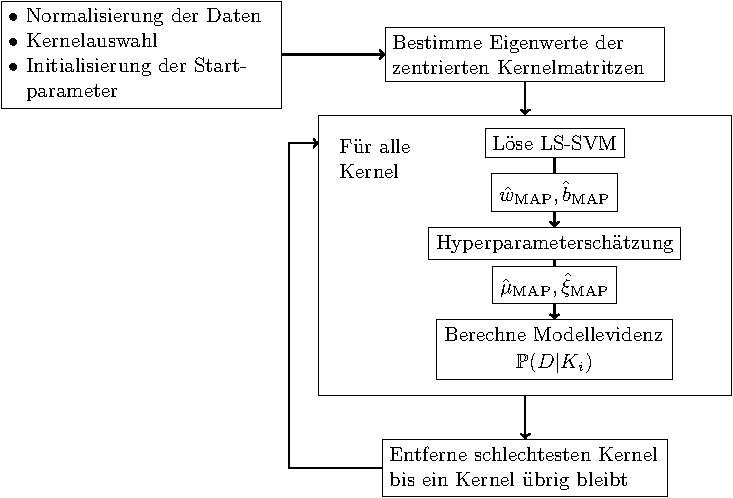
\includegraphics[scale=0.9]{Algo.pdf}
		\caption{Algorithmus zur Kernelselektion bei der LS-SVM}
	\end{figure}
\end{center}

\newpage
\thispagestyle{plain}
\noindent\textbf{Fazit \& Ausblick}\\
Wie wir exemplarisch gezeigt haben, lässt sich die Bayes-Theorie gewinnbringend im Kontext des Machine Learnings verwenden. Der Hauptnutzen besteht darin, numerisch umsetzbare Problemklassen rigoros herleiten zu können. Weiterhin lassen sich Probleme, wie das Hyperparametertuning und die Modellselektion, durch fundierte Ansätze statt bloßer Heuristik angehen. An diesem Punkt stellt sich uns die Frage, aus welchem Grund diese Art von Ansätzen selten in der Praxis Verwendung findet. Gründe hierfür könnten zum einen sein, dass für jedes individuelle Problem eine eigenständige Bayesianische Analyse nötig ist, was zeit- und arbeitsaufwändig ist. Zum anderen könnte es daran liegen, dass die Mischung aus Statistik und Numerik als Schnittstellenbereich zu wenig Aufmerksamkeit bekommt, und deshalb nicht verbreitet ist. Und schlussendlich kann es natürlich auch sein, dass uns nicht bekannte Nachteile bei den verwendeten Ansätzen bestehen. Im Blick auf die Zukunft des Machine Learnings wäre eine Grundlagentheorie und eine detaillierte, mathematisch saubere Untersuchung der zugrunde liegenden Prinzipien wichtig. Die Bayes-Theorie kann hierzu das mathematische Bindeglied zwischen der Statistik, der Numerik und Data Science sein. Da die Probleme und Prinzipien des Machine Learning von Natur aus ein holistisches Denken verlangen, wird eine Zusammenarbeit dieser Sparten zunehmend immer wichtiger.

\newpage
\nocite{*}
\bibliographystyle{plain}
\bibliography{papers}

\end{document}